\documentclass[10pt]{article}
\usepackage[margin=0.75in]{geometry}
\usepackage{tikz}
\usepackage{amsmath}
\usepackage{enumitem}
\usepackage{color,soul}

\usepackage{multicol}

\newcommand{\ds}{\displaystyle}

\begin{document}
\newcounter{enumCount}
\pagestyle{empty}
\subsubsection*{Math 105 - Homework 7 \hfill Name: \underline{\hspace*{2in}}}
\textit{The following problems are organized by the concepts they use.  You should try to solve each problem without any outside help (no computers, calculators, etc.).}

\subsubsection*{Factoring} 

{\color{blue}Know the two kinds of factoring: factoring out \textbf{common factors} and factoring \textbf{quadratic polynomials}.} \\
\textit{Simplify the following expressions as much as possible by factoring.}
\begin{multicols}{2}
\begin{enumerate}
\item $x^2 - 7x + 10$
\item $x^2 (x-5) - 4 (x- 5)$
\setcounter{enumCount}{\theenumi}
\end{enumerate}
\end{multicols}
\vfill

\subsubsection*{Fraction Operations} 

{\color{blue}Understand how to add, subtract, multiply, and divide fractions.} \\
\textit{Simplify each of the following to a single reduced fraction}
\begin{multicols}{2}
\begin{enumerate}
\setcounter{enumi}{\theenumCount}
\item $\dfrac{4}{x-3} - \dfrac{7}{x(x-3)}$
\item $\dfrac{\dfrac{1}{x+h} - \dfrac{1}{x-h}}{\dfrac{h}{2}}$
\setcounter{enumCount}{\theenumi}
\end{enumerate}
\end{multicols}
\vfill

\subsubsection*{Cancellation Rules} 

{\color{blue}You can cancel \textbf{common factors} in fractions, but not terms!} \\
\textit{Simplify as much as possible.}
\begin{multicols}{2}
\begin{enumerate}
\setcounter{enumi}{\theenumCount}
\item $\dfrac{x^2 - 2x + 1}{x^2 + 3x - 4}$
\item $\dfrac{6x^4}{x^4 + x^2}$
\setcounter{enumCount}{\theenumi}
\end{enumerate}
\end{multicols}
\vfill


\subsubsection*{Distribution, FOIL, and Order of Operations} 


{\color{blue}Use distribution and the FOIL method to expand products of factors into sums of terms.} \\
{\color{blue}Know the correct order of operations (PEMDAS or GEMS).} \\
\textit{Expand the following expressions.}
\begin{multicols}{2}
\begin{enumerate}
\setcounter{enumi}{\theenumCount}
\item $2 + x(x-3)(2x+1)$
\item $y + 2(y - 4(x - 1))$
\setcounter{enumCount}{\theenumi}
\end{enumerate}
\end{multicols}
\vfill
 
\newpage
\subsubsection*{Solving Polynomial and Rational Equations} 


{\color{blue}Solve polynomial equations by moving every term to one side and factoring.} \\
{\color{blue}A fraction is only zero when the top is.} \\
\textit{Find all solutions to the following equations.}
\begin{multicols}{2}
\begin{enumerate}
\setcounter{enumi}{\theenumCount}
\item $6x = x^2 + 8$
\item $\dfrac{x^3 + 6x^2 + 5x}{x - 1} = 0$
\setcounter{enumCount}{\theenumi}
\end{enumerate}
\end{multicols}
\vfill


\subsubsection*{Solving Simple (Non-Polynomial) Equations} 
{\color{blue}You can do anything you want, as long as you do it to both sides.} \\
\textit{Solve each of the following equations for $x$. }
\begin{multicols}{2}
\begin{enumerate}
\setcounter{enumi}{\theenumCount}
\item $5 = \dfrac{30}{x-4}$
\item $5y = \dfrac{30}{x-4}$
%\item $y = \sqrt{3x - 4}$
\setcounter{enumCount}{\theenumi}
\end{enumerate}
\end{multicols}
\vfill

\subsubsection*{Functions and Graphs} 
{\color{blue}Understand function notation and how graphs relate to functions.} \\
{\color{blue}Understand linear functions and slope.} \\
\textit{Graph the following functions. Label the points where they cross the $x$ and $y$-axes.}
\begin{multicols}{2}
\begin{enumerate}
\setcounter{enumi}{\theenumCount}
\item $f(x) = \dfrac{x^2 - 4x - 5}{5}$
\item $g(x) = -\tfrac{1}{2}(x-2) + 1$
\setcounter{enumCount}{\theenumi}
\end{enumerate}
\end{multicols}
\vfill
\vfill
\vfill


\begin{enumerate}
\setcounter{enumi}{\theenumCount}
\item Use the graph below to find the values of $x$ for which $f(x) > -3.$ 
\end{enumerate}
\begin{center}
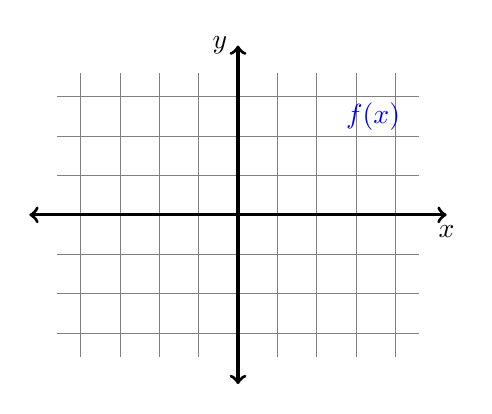
\begin{tikzpicture}[scale=0.5]
\draw[black!50,very thin] (-4.6,-3.6) grid (4.6,3.6);
\draw[very thick,<->] (-5.3,0) -- (5.3,0) node[below] {$x$};
\draw[very thick,<->] (0,-4.3) -- (0,4.3) node[left] {$y$};
\draw[very thick,color=blue] plot[domain=-2:2,samples=100] function {3-3*x**2/4};
\draw[very thick,color=blue,<-] plot[domain=-3.2:-2,samples=100] function {3*(x+2)};
\draw[very thick,color=blue,->] plot[domain=2:4.5,samples=100] function {12/x-6};
\draw (2.5,2.5) node[blue, right] {$f(x)$};
\end{tikzpicture}
\end{center}

\end{document}
